\subsection{Sekvensdiagrammer (Magnus)}
Dette afsnit indeholder 4 sekvensdiagrammer for udvalgte user stories fra sektion 1.4. De 4 sekvensdiagrammer fokuserer på:

\begin{enumerate}
    \item Projektleder opretter projekt.
    \item Medarbejder søger assistance hos en anden medarbejder.
    \item Medarbejder registrerer timer arbejdet.
    \item Medarbejder opdaterer sin status.
\end{enumerate}
    
\begin{figure}[H]
    \centering
    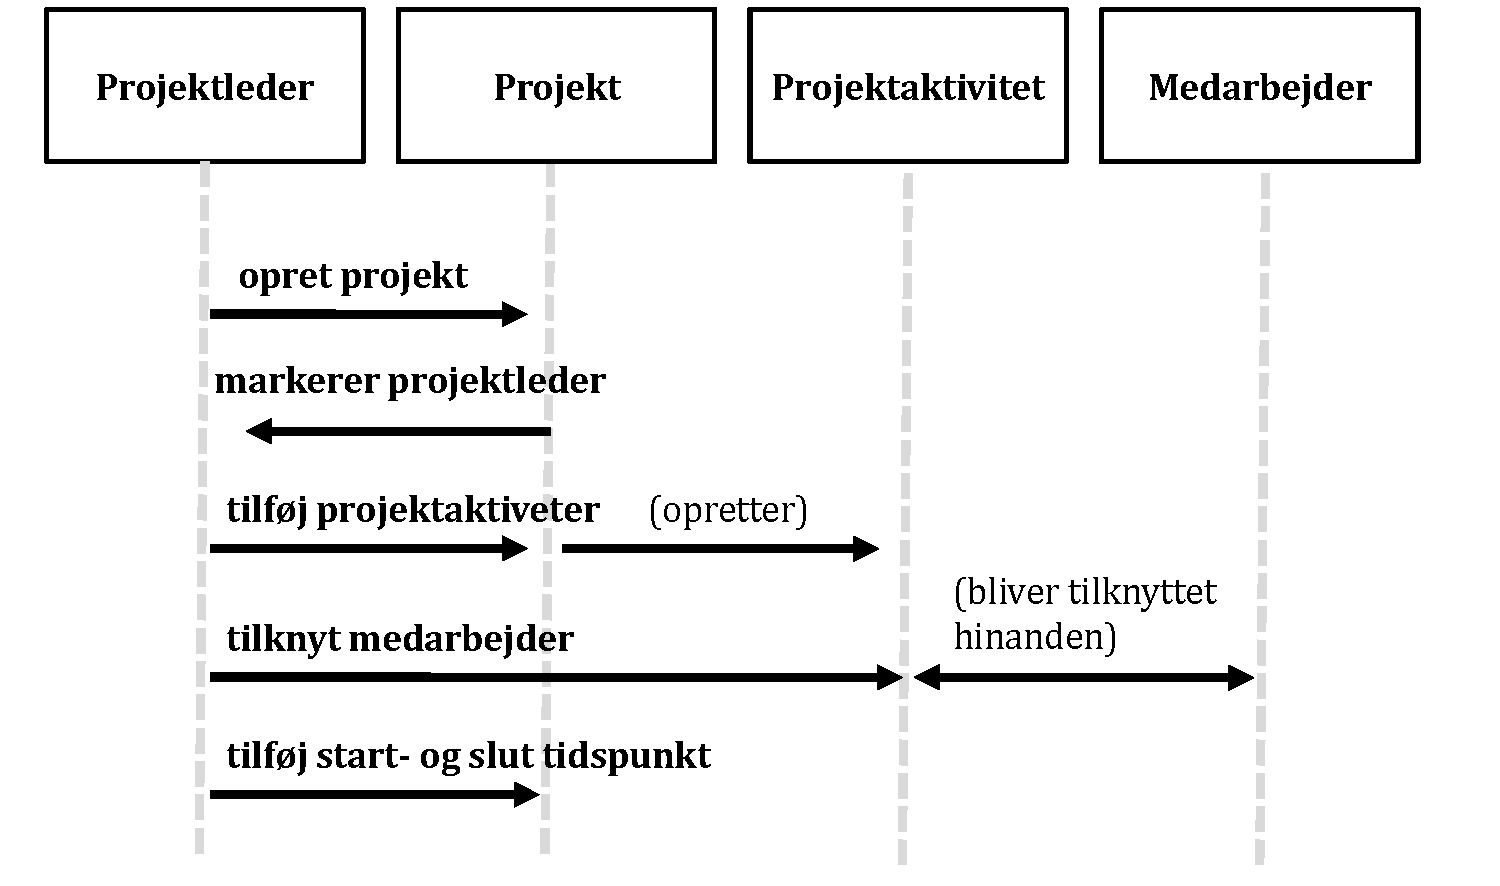
\includegraphics[width=\textwidth]{Figurer/seq1_opretprojekt.pdf}
    \caption{Sekvensdiagram for user stories: "Medarbejdere skal kunne oprette projekter", "Projektledere skal kunne tilføje aktiviteter", "projektledere skal kunne bemande et projekt", "Projektledere skal kunne tilføje projekters start- og sluttidspunkt".}
    \label{fig:seq1_opretprojekt}
\end{figure}

\begin{figure}[H]
    \centering
    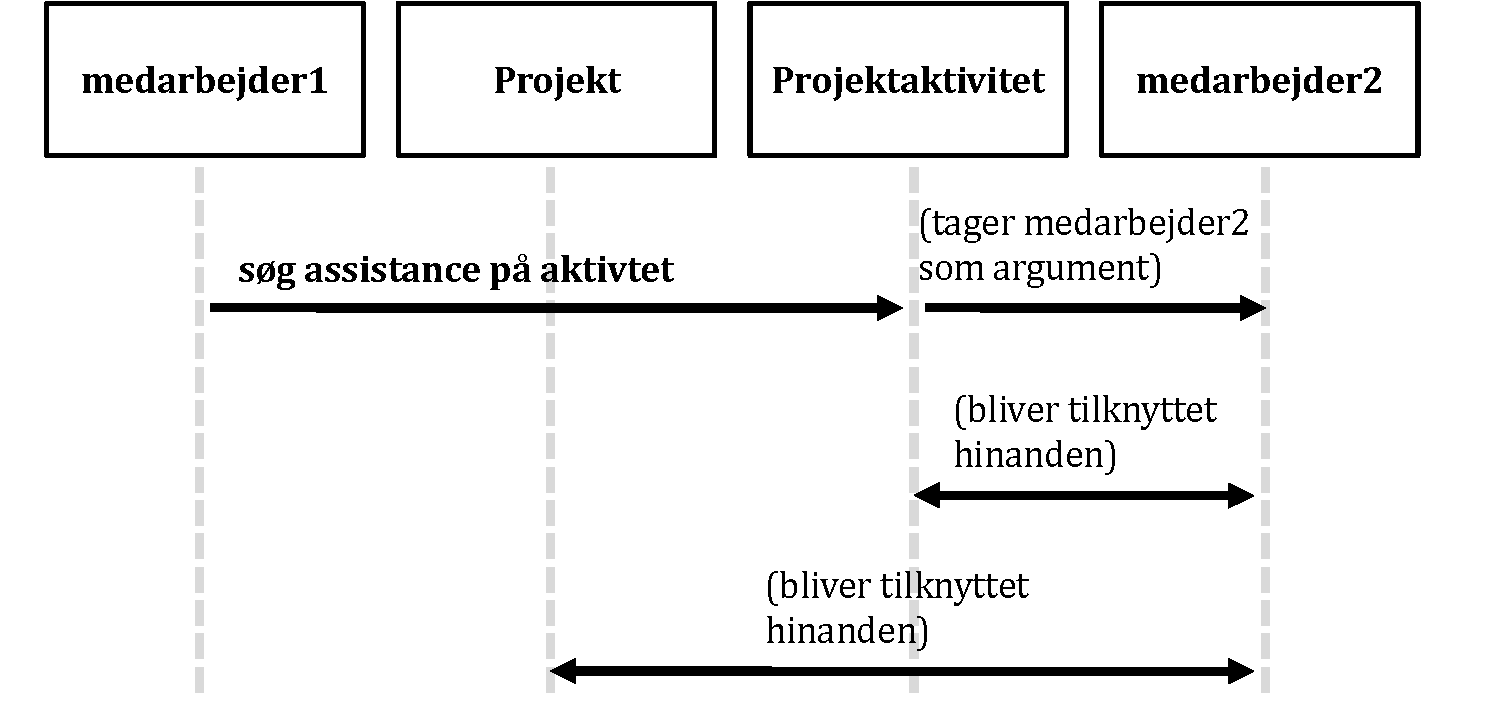
\includegraphics[width=\textwidth]{Figurer/seq2_assistance.pdf}
    \caption{Sekvensdiagram for user story: "Medarbejdere skal være i stand til at søge hjælp hos en kollega".}
    \label{fig:seq2_assistance}
\end{figure}

I praksis er det en medarbejder, der opretter projektet. Medarbejderen markeres dog som projektleder for projektet, idet projektet oprettes.

\begin{figure}[H]
    \centering
    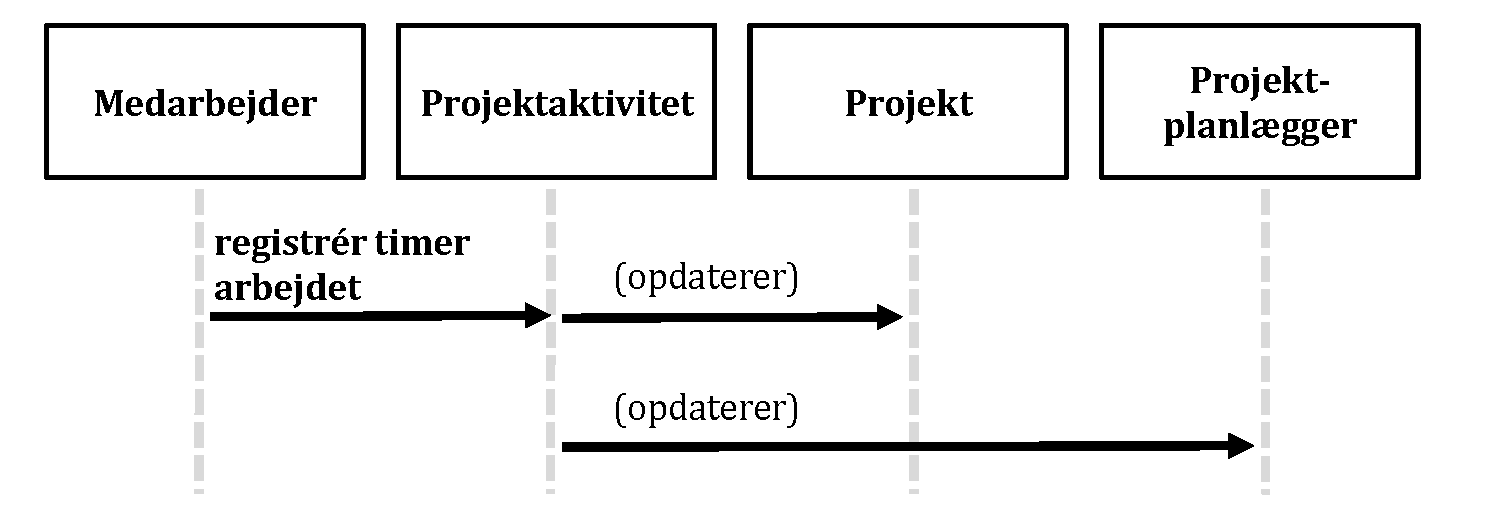
\includegraphics[width=\textwidth]{Figurer/seq3_regtimer.pdf}
    \caption{Sekvensdiagram for user story: "Det skal være muligt for en medarbejder at redigere hvor mange timer han/hun har brugt på hver af personens tilmeldte aktiviteter".}
    \label{fig:seq3_regtimer}
\end{figure}

\begin{figure}[H]
    \centering
    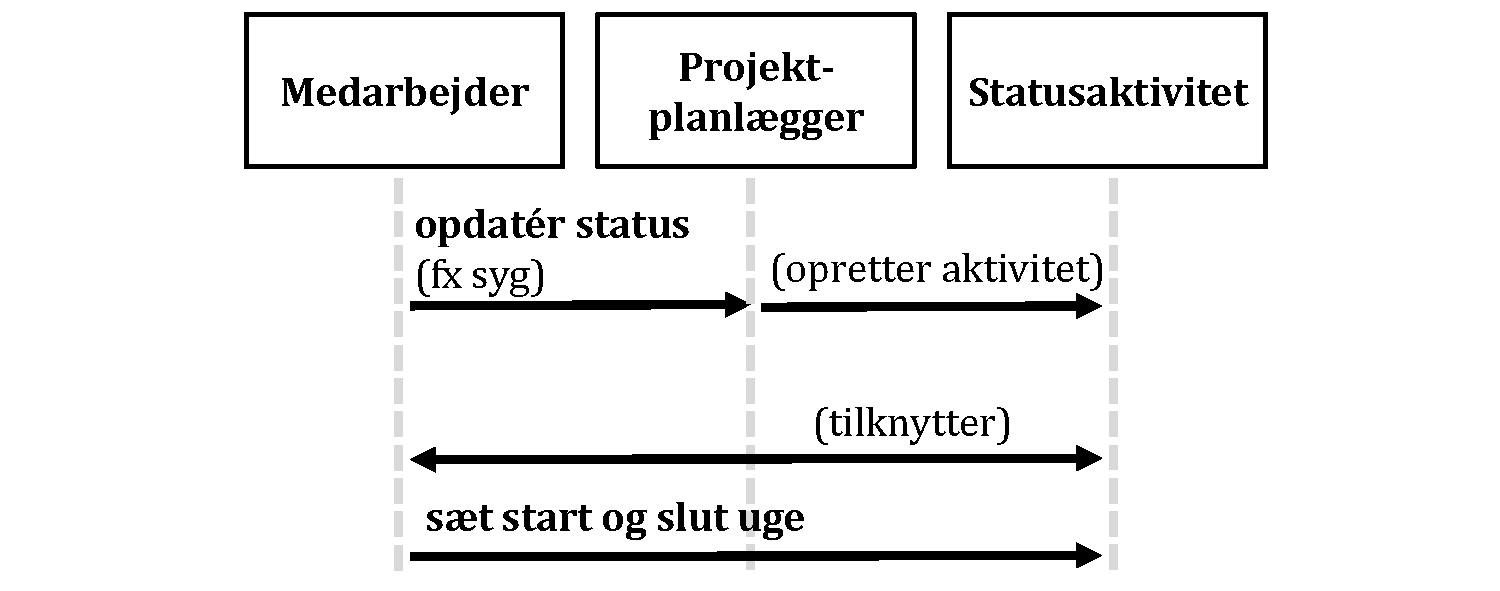
\includegraphics[width=\textwidth]{Figurer/seq4_status.pdf}
    \caption{Sekvensdiagram for user story: "En medarbejder kan tilmelde sig statusaktiviteter som henvender sig til han/hendes erhvervsmæssige  tilstedeværelse".}
    \label{fig:seq4_status}
\end{figure}